\documentclass[a0]{sciposter}
\usepackage[width = 84.10cm, height = 118.90cm, left = 0cm, right = 2.12cm, top = 0cm, bottom = 0cm]{geometry}

\usepackage[english]{babel}
\usepackage[utf8]{inputenc}

\usepackage{graphicx}
\usepackage{ulem}

\definecolor{BoxCol}{RGB}{229,229,229}
\definecolor{HeadCol}{RGB}{30,100,200}

\usepackage{multicol}
\setlength{\columnseprule}{0pt}
\setlength{\columnsep}{1.75cm}

\begin{document}
\vspace*{-2cm}\hspace*{-2cm}
\includegraphics[width = 14.47cm, height = 6.2cm]{logos/icon_UGent_LW_EN_RGB_2400_color.png}

\colorbox{BoxCol}{
\begin{minipage}[t][102cm][t]{82cm}

\vspace{2cm}\hspace{2cm}\begin{minipage}[t]{77cm}
{\fontsize{50}{52}\selectfont\textcolor{HeadCol}{\uppercase{BantUGent - UGent Centre for Bantu Studies}}}
\bigbreak\bigbreak
{\fontsize{40}{44}\selectfont{\textbf{Dirk Seidensticker, Bernard Clist, Wannes Hubau, Hans Beeckman, Koen Bostoen, Sara Pacchiarotti}}}
\bigbreak\bigbreak
{\fontsize{44}{50}\selectfont\textcolor{HeadCol}{\uline{\textbf{\uppercase{The Late Holocene Settlement History of the Central African Rainforest:}}}}}
\bigbreak
{\fontsize{44}{50}\selectfont\textcolor{HeadCol}{\uline{\textbf{\uppercase{Archaeological, Palaeoenvironental and Linguistic Evidence for 3,000 years of}}}}}
\bigbreak
{\fontsize{44}{50}\selectfont\textcolor{HeadCol}{\uline{\textbf{\uppercase{Interaction between Bantu Speech Communities and their Changing Environments}}}}}
\end{minipage}

\vspace{2cm}\hspace{2cm}\begin{minipage}[t]{24.5cm}
{\fontsize{28}{36} \selectfont During the past forty years, archaeology in the Central African rainforest has made a significant contribution to our understanding of the settlement history of one of Africa's major biotopes. Taking into account the massive extent of this biotope, the promising results of past research, which filled the blank spot that the rainforest presented on any archaeological distribution map of Africa until the 1970s, can only be seen as starting points. Our poster aims at reviewing our current knowledge on the settlement history of the Central African rainforest as it has been documented through surveys and excavations as well as through the late Holocene paleo-environmental record between present-day Cameroon and Angola.}
\bigbreak
{\fontsize{28}{36} \selectfont The earliest traces of sedentary and potentially food producing peopling, mainly identified through pottery finds, date into the first millennium BC and are commonly seen in relation to a contemporaneous crisis of the rainforest and to the expansion of Bantu languages and their speech communities.}
\end{minipage}

\vspace{5cm}
\hspace{2cm}\begin{minipage}[t]{77cm}
\begin{multicols}{3}

{\fontsize{38}{42} \selectfont \textcolor{HeadCol}{Archaeology}}
\bigbreak
{\fontsize{28}{36} \selectfont The archaeological record of Central Africa must be divided into two blocks of research (Fig. 1). The western or coastal area, characterized by a diverse history of research, and the Congo Basin, whose archaeological record goes back to the River Reconnaissance Project led by Manfred Eggert. The latter derived a remarkably coherent dataset covering the last two and a half millennia.}
\bigbreak
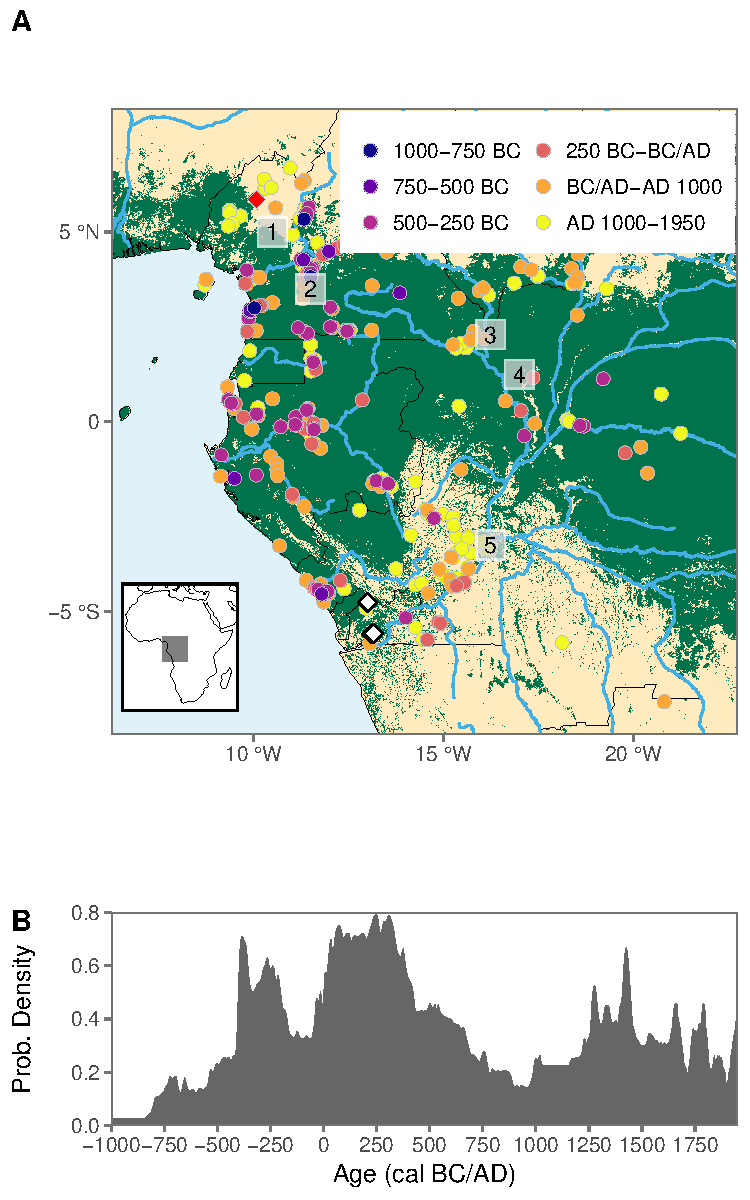
\includegraphics[width = \linewidth]{img/FigArch.pdf}
\bigbreak
{\fontsize{28}{36} \selectfont Results from the Congo Basin indicate a diverse, non-uniform settlement history. A site activity curve (Fig. 2 A) indicates lesser amount of settled sites within the Early Iron Age (400 BC–AD 600), followed by a Middle Iron Age recess and a twin-peaked Late Iron Age (from AD 1100).1 The group dispersion calibration of 684 late Holocene radiocarbon dates from the Central African rainforest (Fig. 2 B) illustrates both a diverse settlement history and a research bias, focussing on the Early Iron Age.}
\bigbreak
{\fontsize{28}{36} \selectfont Recent studies in the north-eastern parts of the Congo Basin show a distinct change in technological as well as stylistic attributes of the pottery that might be associated with a possible demographic change (Livingstone-Smith et al. 2017). Similar changes have been observed along the Sangha river and are dated towards the 13th c. AD (Seidensticker in Prep.).}
\vfill\null
\columnbreak
{\fontsize{38}{42} \selectfont \textcolor{HeadCol}{Paleoecology}}
\bigbreak
{\fontsize{28}{36} \selectfont Palaeobotanical evidence showed that climatic anomalies had an impact on Central African vegetation. Intense droughts are thought to leave the forest structure severely fragmented. This particularly happened during the third millennium BP rainforest crisis (3MBP, 3-2 ka BP) and the Medieval Climate Anomaly (MCA, 1.1 - 0.7 ka BP). Both periods are characterized by increasing sea surface temperatures (SST) near the Congo River mouth. Peaks in SST are associated with drought periods on the Central African continent. During these periods, contiguous forest areas were turned into mosaics of forest and savanna patches.}
\bigbreak
{\fontsize{28}{36} \selectfont Although climate-driven forest disturbance certainly occurred during drought periods throughout the Holocene, migrating Bantu-speaking farmers may have enhanced the process of forest destruction. Bantu people started migrating south from their cradle near the Niger delta some 4000 years ago, due to aridification of their Sahel farmland. By applying slash-and burn techniques in rainforest areas, they may have significantly contributed to forest fragmentation. However, while human impact was probably an important factor during the last millennium, it is still unclear how significant their role was during the 3rd millennium rainforest crisis.}

\vfill\null
\columnbreak
{\fontsize{38}{42} \selectfont \textcolor{HeadCol}{Linguistics}}
\bigbreak
{\fontsize{28}{36} \selectfont Recent lexicon-based phylogenetic studies show that two parallel Bantu subclades, Congo Bantu (CB) and West-Coastal Bantu (WCB), split off of their ancestor clade North-Western Bantu (NWB) possibly around date xx?. Their pre-split off homeland was probably somewhere in the current border region between Cameroon, Gabon, the Congos and the CAR (in the middle of the Sangha River Interval, SRI).}
\bigbreak
INSERT RELEVANT PORTION OF TREE FIGURE HERE?
\bigbreak
{\fontsize{28}{36} \selectfont The first Central African forest crisis resulting in savannah extension on its periphery around 4000 BP likely facilitated the slow pace migration of the ancestors of NWB speakers from their homeland in the Cameroonian Grassfields southwards into the Sanaga-Mbam confluence area, a fact also confirmed by archaeological evidence.}
\bigbreak
{\fontsize{28}{36} \selectfont On the other hand, the second Central African forest crisis, which perturbed its core around 2500 BP and caused a reopening of the Sangha River Interval (SRI), boosted rapid and large-scale longitudinal expansions of the ancestors of CB and WCB speakers from their homeland in the midst of the SRI. The corridor created by the reopening of the SRI favored the rapid southward expansion of WCB speakers into the area straddling the Batéké Plateau and the Bandundu region (DRC), as well as the eastward expansion of CB speakers toward the Congo-Ubangi confluence area.}
\bigbreak
INSERT A MODIFIED VERSION OF FIG. 2 IN 2015 PAPER HERE?
\bigbreak
{\fontsize{28}{36} \selectfont However, the tentative WCB homeland somewhere close to the Batéké Plateau, resulting from ancestral speakers fastly moving southwards around 2500 BP, is at odds with Tchissanga pottery found on the Congolese Atlantic coast dating 2500-2200 PB, the oldest tradition within present-day borders of WCB. This paradox might have two explanations: either older ceramic traditions will be found in the archaeologically unexplored Batéké Plateau area, or coastal Tchissanga pottery producers spoke a non-WCB language(s).}

\vfill

\end{multicols}
\end{minipage}
\end{minipage}}

\hspace*{-2cm}
\includegraphics[width = 10.51cm, height = 8.41cm]{logos/logo_UGent_EN_RGB_2400_color.png}
%\begin{tabular}{cccc}
% & 
\includegraphics[width = 7.05cm, height = 4.7cm]{logos/logo_tervuren_horizontaal.jpg} & International Conference Climates and Cultures: Perspectives for the Future & 23-24 May 2018
%\end{tabular}  

\end{document}